\chapter{Corrected NBC}

In the previous section we considered the maximum likelihood estimate for the probabilities required in the NBC.
We saw that our classifier fails to classify an object with attribute $a_j$ and class $c$ if there are no previous observations of this combination in our training data set.
In this chapter we will define our prior distribution which will form the basis for the naive Credal classifier we discuss later.
The prior we will use is the same prior as that used by Zaffalon when constructing the naive Credal classifier \cite{Zaffalon01}.
Once again we will not be introducing any new ideas, however we will discuss areas for further investigation.

\section{Introducing a Prior}
The problem of zero frequencies is especially common in the field of language modelling \cite{Chen96}.
Standard practice in language modelling is to break a sentence down in to individual words.
The aim is to then estimate the probability of encountering a certain word in text.
However due to the large number of words in a language, and the limited size of the data set, the maximum likelihood estimate for many words will be zero.
One such approach to this problem is to add a small pseudocount to each word, which is known as additive smoothing \cite{Manning08}.
This is the same as adding a prior distribution to our probability estimates.

We return to our likelihood function for our $\bm{\theta}$ variables \cref{likelihood}.
We will introduce a prior distribution for these parameters and then consider the posterior distribution.

The Dirichlet distribution is the multinomial extension of the beta distribution for $\theta_1,\dots,\theta_k$ where $\theta_i \in (0,1)$ and $\sum_{i=1}^k \theta_i = 1$ with probability density function:
\begin{equation} \label{dirichlet_pdf}
	f(\theta_1,\dots,\theta_k \mid s, t(1),\dots,t(k)) \propto \prod_{i=1}^k \theta_i^{st(i) - 1}
\end{equation}
where $s > 0$ and each $t(i)>0$ such that $\sum_{i=1}^{k}t(i) = 1$.
The family of Dirichlet distributions is a conjugate prior for the multinomial distribution.

We introduce a distribution that has similar properties to the Dirichlet distribution and has a similar structure to our likelihood as our prior density:
\begin{equation} \label{prior}
	f(\bm{\theta} \mid \mathbf{t}, s) \propto \prod_{c \in \mathcal{C}} \left[ \theta_c^{st(c) - 1} \prod_{i=1}^k \prod_{a_i \in \mathcal{A}_i} \theta_{a_i \mid c}^{st(c, a_i) - 1} \right]
\end{equation}
This is in the same form as the likelihood however each $n(\cdot)$ is replaces by $st(\cdot) - 1$.
$s > 0$ is a fixed constant and we have the following constraints on $t(\cdot):$
\begin{align}\label{prior_constraints}
	\sum_{c \in \mathcal{C}} t(c) & = 1 \\
	\sum_{a_i \in \mathcal{A}_i} t(a_i, c) & = t(c) && \forall i, c \\
	t(a_i, c) & > 0 && \forall i, a_i, c
\end{align}
These constraints retain the structure seen for the frequencies in our likelihood.

This family of distributions is a conjugate prior for the likelihood function \cref{likelihood}.
When we multiply our likelihood by a prior density of this form we get a posterior in the same family as the prior.
If the prior has hyperparameters $st(\cdot)$ the posterior will have hyperparameters $st(\cdot) + n(\cdot)$.
The conjugate prior make the posterior more convenient to handle and also allows us to directly observe how the likelihood updates the prior.

We can now estimate the parameters by taking the posterior expectation:
\begin{align}
	E[\theta_c \mid \mathbf{n},s,\mathbf{t}] & = \frac{n(c) + st(c)}{N + s} = \hat{\theta}_c \\
	E[\theta_{a_i \mid c} \mid \mathbf{n},s,\mathbf{t}] & = \frac{n(a_i, c) + st(a_i, c)}{n(c) + st(c)} = \hat{\theta}_{a_i \mid c}
\end{align}

Note that if we observe more vehicles from the population we do not expect the ratios to tend to these estimated probabilities.
These estimates represent the proportions of vehicles from all possible populations from which we could have drawn our original data set \cite{Lidstone20}.

\section{Prior Distribution Hyperparameters}

To apply this classifier to our data set we need to choose the hyperparameters of the prior distribution.

We note that $s$ represents the strength of our prior distribution when calculating the posterior and hence determines how quickly our classifier learns from the observed data.
As $s \rightarrow 0$ we get the maximum likelihood estimates.
On the other hand if $s$ is extremely large the observed frequencies are dominated by our prior beliefs.
Walley recommends setting $s=1$ or $s=2$ as these are considered ``reasonably cautious'' \cite{Walley96}.
When comparing the NBC to the corrected NBC we will set $s=1$.
We will then look at the sensitivity of the corrected NBC with respect to the $s$ value.

The other hyperparameters $t(\cdot)$ represent our prior beliefs for $P(\cdot)$.
Initially we have no information regarding what these probabilities are and Laplace tells us \cite{Laplace1812} the best way to represent this is by making them all equal in our prior.
This is referred to as ``the principal of indifference'' by Keynes \cite{Keynes21} who criticised it as a representation of a lack of prior information.
He presented several situations where this principal leads to paradoxes.

In this section we will follow the principal of indifference when selecting our prior distribution.
However we will address this problem in chapter 4 where we introduce the imprecise prior.
Hence we set:
\begin{align}\label{initial prior}
	t(c)      & = \frac{1}{|C|} \\
	t(a_i, c) & = \frac{1}{|A_i||C|}
\end{align}
These assignments obey the constraints given in \cref{prior_constraints}.

\section{Comparison to Uncorrected NBC}

% Seed = 0.5

Setting $s=1$ and using 10-fold cross validation the accuracy and percentage of indeterminate classifications are shown below:
\begin{center}
	\begin{tabular}{ c|c c }
		              & Accuracy & Indeterminate Classifications \\
		\hline
		NBC           & 63.73\%  & 18.13\%                       \\
		Corrected NBC & 69.43\%  & 0\%
	\end{tabular}
\end{center}

In addition we can consider the confusion matrix:
\begin{center}
    \begin{tabular}{l l r r r r r r}
    \hline
                       &    & \multicolumn{6}{c}{Predicted Class}                   \\
    \hline
                       &    & -2      & -1    & 0       & 1       & 2       & 3     \\
    \hline
    \multirow{6}{*}{Actual Class} & -2 & \textbf{0.0\%}  & 1.55\% & 0.0\%   & 0.0\%   & 0.0\%  & 0.0\%  \\
                       & -1 & 1.55\% & \textbf{5.7\%}   & 3.63\%  & 0.52\%  & 0.0\%  & 0.0\%  \\
                       & 0  & 0.0\%  & 1.55\% & \textbf{24.87\%}  & 4.66\%  & 1.55\% & 0.0\%  \\
                       & 1  & 0.0\%  & 2.59\% & 2.07\%  & \textbf{19.17\%}  & 1.04\% & 1.55\% \\
                       & 2  & 0.0\%  & 0.0\%  & 1.55\%  & 2.07\%  & \textbf{11.4\%}  & 1.04\% \\
                       & 3  & 0.0\%  & 0.0\%  & 0.52\%  & 0.52\%  & 2.07\% & \textbf{8.81\%} \\
    \hline
    \end{tabular}
\end{center}

Using posterior expectations instead of maximum likelihood estimates improves our classifier in all three metrics.

We can also see that our classifier rarely assigns risk ratings that are far away from the true risk rating.
For example if the risk rating is 2 or 3 our classifier never assigns a negative risk rating.
In the next section we will look to see whether we can reduce this further.

Introducing the prior distribution means that we no longer have indeterminate classifications as $P(c \mid \mathbf{a})$ will never be zero.
We will investigate how sensitive our classifier is to our choice of prior hyperparameters.

A proportion of vehicles that previously had indeterminate classifications are now classified correctly.
This has led to an increase in the accuracy of our classifier.
However we are still achieving an accuracy of less than 70\% which still leaves room for improvement.

\section{Varying $s$ Hyperparameter}

We now look at the sensitivity of the accuracy of the corrected NBC to changes in the $s$ hyperparameter.
If we choose $s$ values log uniformly between $10^{0}$ and $10^{6}$ and plot these against the accuracy of the corrected NBC we get the following plot:
\begin{center}
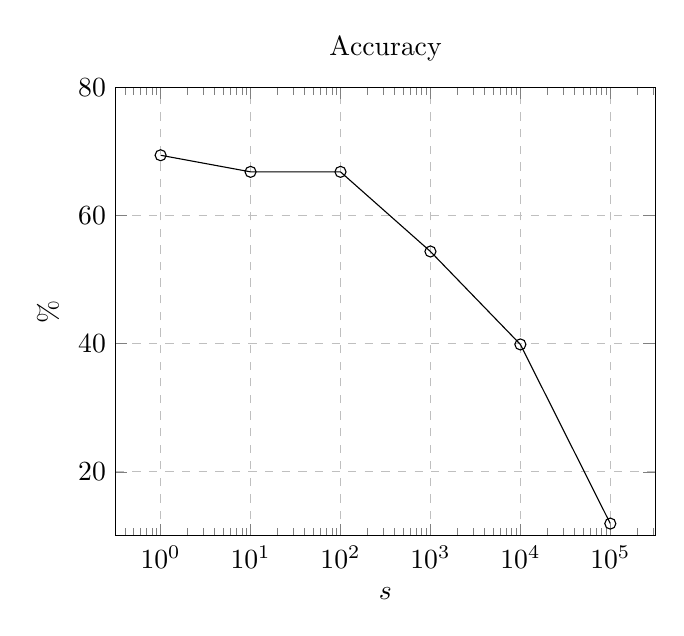
\begin{tikzpicture}
\begin{axis}[
    title={Accuracy},
    xlabel={$s$},
    ylabel={\%},
   	xmode = log,
    ymin=10, ymax=80,
    ymajorgrids=true,
    xmajorgrids=true,
    grid style=dashed,
]

\addplot[
	mark=o,
    color=black,
    ]
    coordinates {
    (1,69.430)
    (10,66.839)
    (100,66.839)
    (1000,54.404)
    (10000,39.89)
    (100000,11.917)
    };
 
\end{axis}
\end{tikzpicture}
\end{center}

The most obvious feature is the significant drop in accuracy between $s=100$ and $s=10000$.
This is where the prior dominates the likelihood and the posterior expectations for the probabilities become uniform.
For large $s$ our classifier assigns classes at random uniformly.

On the other side of the graph, for $s=1$ we see a fairly consistent classifier with accuracy of about 70\%.

We have seen that the corrected NBC has a greater accuracy than the normal NBC and never returns indeterminate classifications.
We have also seen the effect varying the hyperparameter $s$ has on this classifier.

We did not change the choice of decision rule in our classifier or the metrics used to measure how successful our classifier was.
In the next chapter we will make use of the risk rating structure.
The accuracy metric does not take into account how close the classification is.
For example if the true class is 2 an assigned class of 1 should be considered better than an assigned class of -2.
The 0-1 loss function also does not take this into account and a better choice of loss function may prove beneficial.